\chapter{The viscous cylinder}
The flow around a viscous cylinder has been approached by many papers both analytically \todo{wirklich?} and numerically, e.g. \todo{literatur}, though very few numerical approaches use a \gls{rkdg} method combined with immersed boundaries. In order to verify the \gls{bosss} code with immersed boundaries not only for the Euler equations as we did in \ref{eulerVerification} but also for the viscous case we will now consider different Reynolds numbers for the steady and unsteady flow and compare our results to those of other studies.

\section{Theory}
	The flow around a viscous cylinder can be divided in different sections depending on the Reynolds number. The first section applies for a Reynolds number $0 < \text{Re} < 40-50$ characterised by a laminar steady flow. In that regime a recirculation region with two symmetric vortices with opposite directions is comprised by the wake. The flow can be described using the wake separation length $W^*$.\\\\
	\begin{figure}[htp]
		\centering
		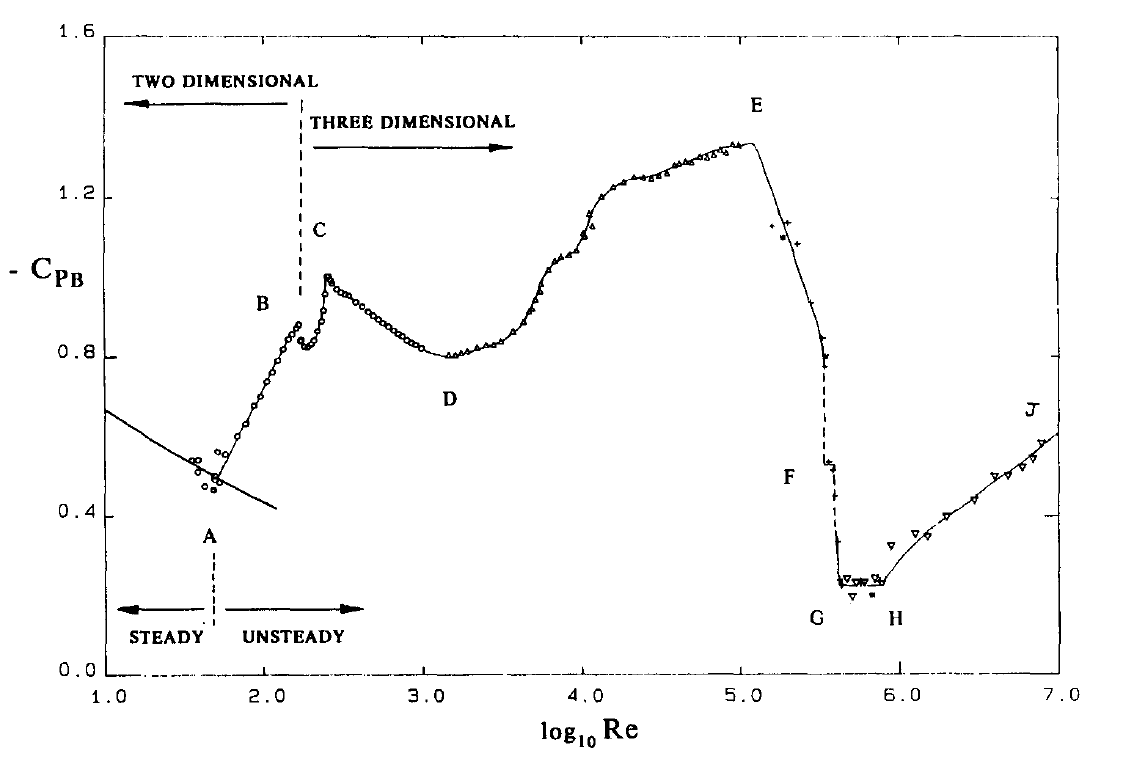
\includegraphics[height=8cm]{overviewCylinderReynolds_Williamson.PNG}
		\caption{Overview of Base Suction Coefficients over Reynolds Number \todo{Quelle}}
		\label{fig:overview}
	\end{figure} 
	The second section contains all other Reynolds number $\text{Re}> 40-50$ and thus describes the unsteady flow. It can be subdivided in several subsections:
	\begin{description}
		\item[$40-50 < \text{Re} < 190$] laminar vortex shedding,
		\item[$190 < \text{Re} < 260$] 3-D wake-transition regime,
		\item[$260 < \text{Re} < 1000$] increasing disorder in the fine-scale three dimensionalities,
		\item[$1000 < \text{Re} < 200000$] shear layer transition regime,
		\item[$200000 < \text{Re}$] critical transition, supercritical regime and post-critical regime.
	\end{description}
	
	As we will only discuss Reynolds numbers up to $\text{Re} < 200$ the important phases for us are the laminar steady regime and the laminar vortex shedding. At around $\text{Re} = 190$ the three dimensionality of the system has a incrementing influence on the flow; for we only analyse the 2-D model of the experiment we stop at $\text{Re} = 200$ expecting slight deflection in our results.
	
	\subsection{The Laminar Steady Regime}
	
		\begin{figure}[htp]
			\centering
			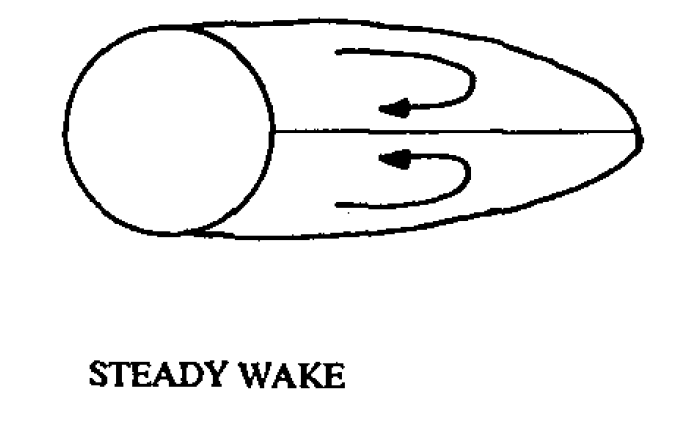
\includegraphics[height=4cm]{steadyFlow_Williamson.PNG}
			\caption{Recirculation Region \todo{Quelle}}
			\label{fig:steady}
		\end{figure}
	\subsection{Laminar Vortex Shedding}
	
		\begin{figure}[htp]
			\centering
			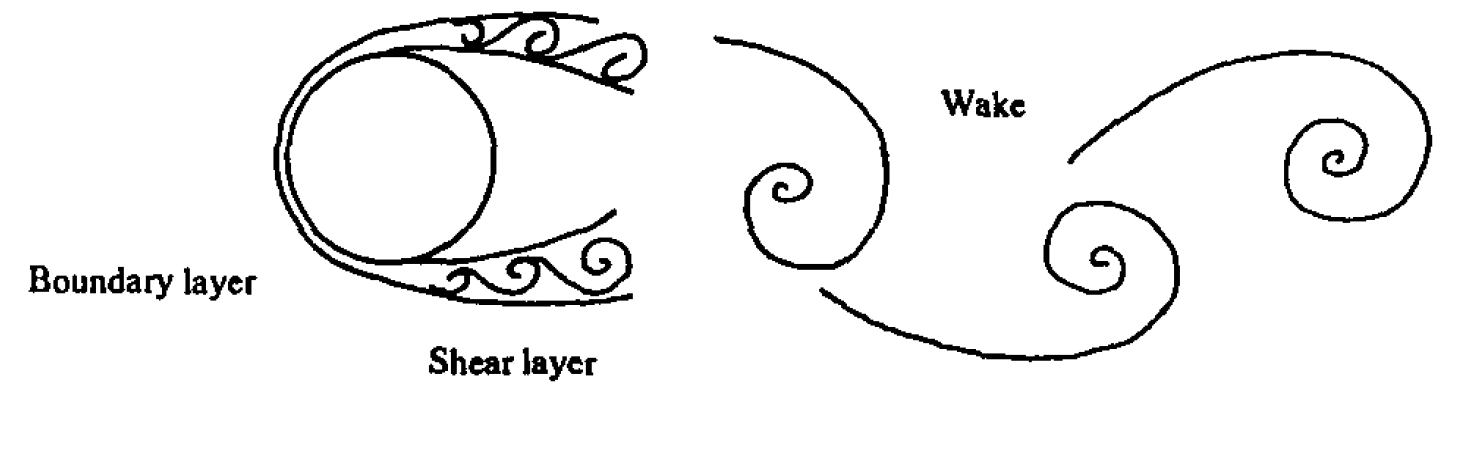
\includegraphics[height=4cm]{unsteady_Williamson.PNG}
			\caption{Karmán Vortex Street \todo{Quelle}}
			\label{fig:unsteady}
		\end{figure}
		
\section{Simulations}
	In this section we will compare the lift and drag coefficients at different Reynolds numbers and mesh sizes at a constant agglomeration threshold of $0.3$ and a polynomial degree of $1$.
	\subsection{Steady State Simulations ($\text{Re} < 40-50$)}
	\subsubsection{Simulation at Reynolds Number 10}
	\subsubsection{Simulation at Reynolds Number 20}
	\subsubsection{Simulation at Reynolds Number 40}
	\subsection{Unsteady Simulations ($\text{Re}> 40-50$)}
	\subsubsection{Simulation at Reynolds Number 100}
	\subsubsection{Simulation at Reynolds Number 200}